\documentclass{article}
\usepackage{amsmath, amssymb, amsfonts}
\usepackage{fullpage}
\usepackage{enumerate}
\usepackage[linesnumbered,ruled,vlined]{algorithm2e}
\usepackage{hyperref}
\usepackage{graphicx}

\title{CS 4780/5780 Homework 8\vspace{-10pt}}
\author{Due: Thursday 29/11/18 11:55pm on Gradescope}
\date{}

\begin{document}
    \maketitle
	\section*{Problem 1:  Trade-off Between Impurity and Tree Size for Regression Trees}
	You are given a dataset $D=\{(-3, -20), (-2, -20), (-1, -17), (0, 15), (1, 25), (2, 26)\}$ and you want to build a regression tree for this dataset.
	\begin{enumerate}
	\item[(a)] Recall that the impurity for the regression tree model is  defined as
	$$
	L(S) = \frac{1}{|S|}\sum_{(x_i, y_i)\in S}(y_i - \bar{y}_S)^2,
	$$
	where $\bar{y}_S = \frac{1}{|S|}\sum_{(x_i, y_i)\in S}y_i$. Draw the regression tree $T_0$ built by ID3-Algorithm which is introduced in the class. (There are multiple correct thresholds. Choose one of them to draw.)
	\item[(b)] We keep the definition of $L(S)$ as (a). Prove that $L(S) \geq \frac{|S_1|}{|S|}L(S_1) + \frac{|S_2|}{|S|}L(S_2)$, where $S_1 \cup S_2 = S$ and $S_1\cap S_2 = \emptyset$. This conclusion tells us the impurity of a regression tree never increases after one split.
	\end{enumerate}
	\textbf{Solution:}
	\begin{enumerate}
	\item[(a)] 
	\begin{figure}
	\centering
	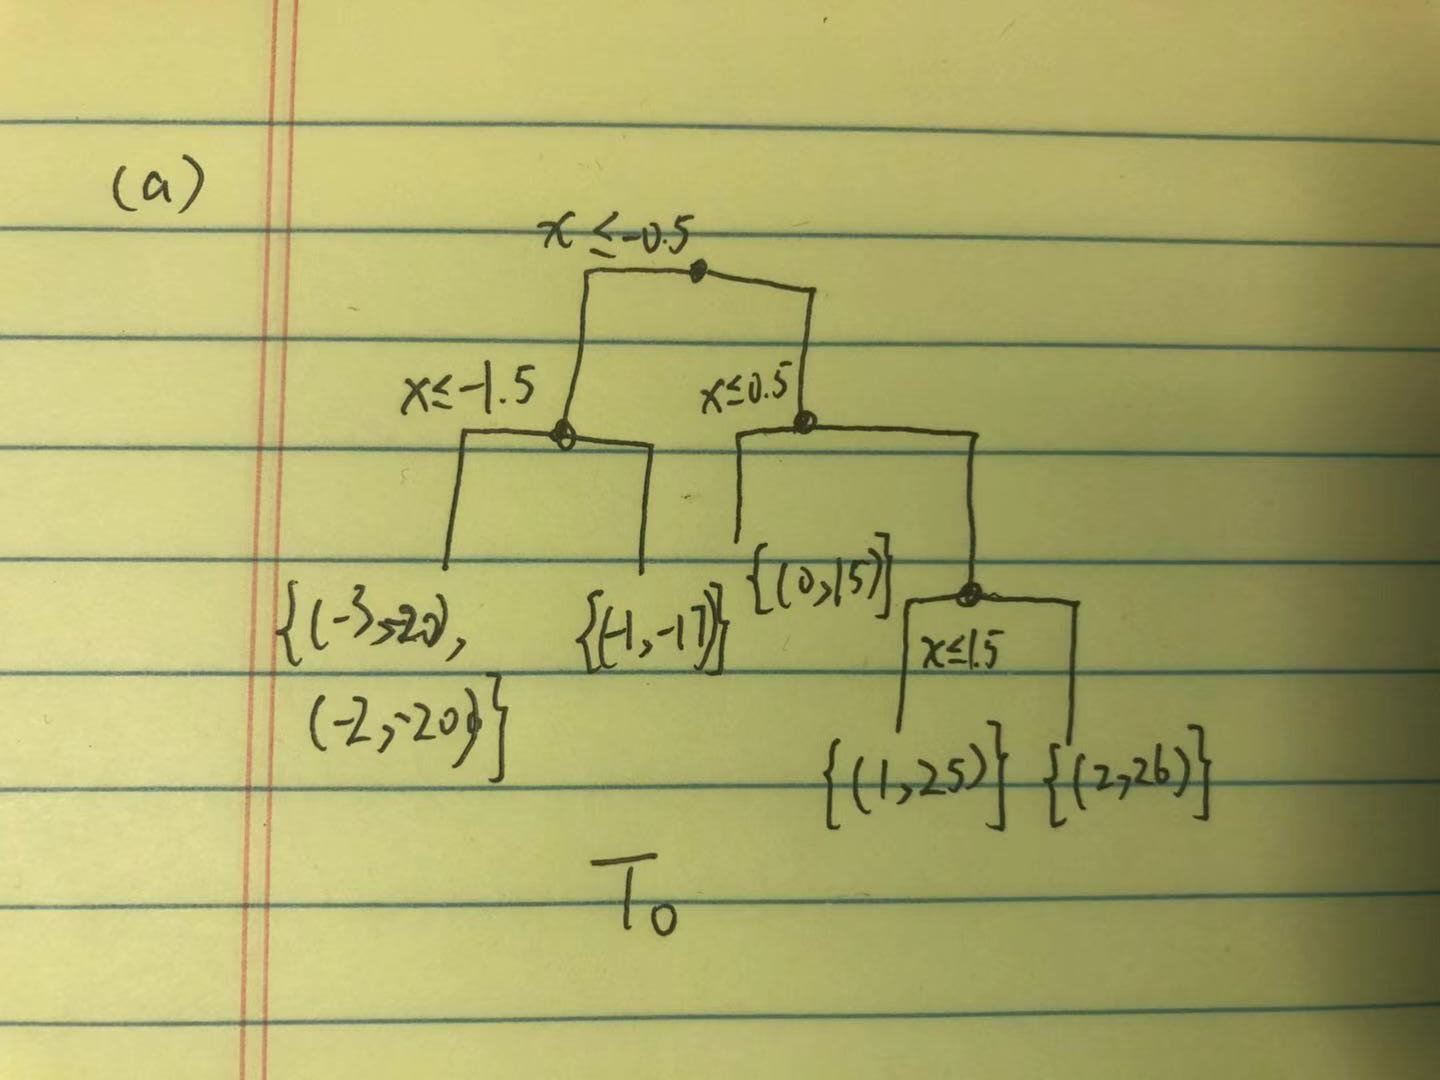
\includegraphics[scale=0.15]{solution1a}
	\label{fig_solua}
	\caption{Solution a}
	\end{figure}
	The tree is shown in Figure \ref{fig_solua}
	
	
	\item[(b)] It's equivalent to show
	$$
	\sum_{(x, y)\in S}(y - \bar{y}_S) \geq \sum_{(x, y)\in S_1}(y - \bar{y}_{S_1})^2 + \sum_{(x, y)\in S_2}(y - \bar{y}_{S_2})^2. 
	$$
	Actually, 
	$$
	\sum_{(x, y)\in S}(y - \bar{y}_S) = \sum_{(x, y)\in S_1}(y - \bar{y}_{S})^2 + \sum_{(x, y)\in S_2}(y - \bar{y}_{S})^2 
	$$
	$$
	\geq \min_{\alpha_1}\sum_{(x, y)\in S_1}(y - \alpha_1)^2 +\min_{\alpha_2} \sum_{(x, y)\in S_2}(y - \alpha_2)^2
	$$
	$$
	=sum_{(x, y)\in S_1}(y - \bar{y}_{S_1})^2 + \sum_{(x, y)\in S_2}(y - \bar{y}_{S_2})^2. 
	$$
	\end{enumerate}
	The proof is done.
	
	
	%\section*{Problem 2:  Ensemble of Independent Models}
	%Given a dataset $D = \{(x_i, y_i)\mid i=1, \cdots, n\}$ where $y_i \in \{+1, -1\}$, you are going to do a classification task by an ensemble model $H$. More specifically,  you are given $2k + 1$ independent models $H_1, H_2, \cdots, H_{2k + 1}$. Each model $H_j$ has probability $p_i$ to make the correct prediction for data $(x_i, y_i)$. We further assume that for each model $H_j$, the predictions for different data are independent. Then $E[\sum_{i=1}^n I[H_j(x_i) = y_i]] = \sum_{i=1}^n p_i$. The ensemble model $H$ is defined as follow:
	%$$
	%H(x_i) =
	%\left\{
	%\begin{array}{rcl}
	%1      &      & {  |\{j\mid H_{j}(x_i) = 1\}| > |\{j\mid H_{j}(x_i) = 0\}| }\\
	%0     &      & { |\{j\mid H_{j}(x_i) = 1\}| < |\{j\mid H_{j}(x_i) = 0\}| }
	%\end{array} \right.
	%$$
	%Prove that $E[\sum_{i=1}^n I[H(x_i) = y_i]] = \sum_{i=1}^n p_i$.
	
	\section*{Problem 2: Normalization Update in Adaboost}
	In the Adaboost, we keep $\sum_{i=1}^n w^i_t = 1$. In the iteration $t$ of the algorithm, we update $w_t^i$ as follow: 
	$$w^i _{t+1}\leftarrow \frac{w^i_t\cdot e^{-\alpha_{t+1} h_{t+1}(x_i)y_i}}{2\sqrt{\epsilon_{t+1}(1-\epsilon_{t+1})}}$$
	where $\alpha_{t+1} = \frac{1}{2}\log \left(\frac{1 - \epsilon_{t+1}}{\epsilon_{t+1}}\right)$ and  $\epsilon_{t+1} = \sum_{i:h_{t+1}(x_i)\neq y_i}w^i_t$. Prove that if $\sum_{i=1}^n w^i_t = 1$, $\sum_{i=1}^n w^i_{t+1} = 1$, i.e. $\sum_{i=1}^{n} w^i_t \cdot e^{-\alpha_{t+1} h_{t+1}(x_i)y_i} = 2\sqrt{\epsilon_{t+1} (1-\epsilon_{t+1})}$. (Remember in the Adaboost, $h_{t+1}(x_i),y_i\in \{+1, -1\}$.) \\
	\\
	\textbf{Solution:}
	$$
	\sum_{i=1}^{n} w^i_t \cdot e^{-\alpha_{t+1} h_{t+1}(x_i)y_i} = \sum_{i=1}^{n} w^i_t \left(\frac{\epsilon_{t+1}}{1 - \epsilon_{t+1}}\right)^{h_{t+1}(x_i)y_i}.
	$$
	Because $h_{t+1}(x_i),y_i\in\{+1, -1\}$, $h_{t+1}(x_i)y_i = 1$ when $h_{t+1}(x_i) = y_i$ and $h_{t+1}(x_i)y_i = -1$ when $h_{t+1}(x_i) \neq y_i$.
	$$
	\sum_{i=1}^{n} w^i_t \cdot e^{-\alpha_{t+1} h_{t+1}(x_i)y_i} = \sum_{i=1}^{n} w^i_t \left(\frac{\epsilon_{t+1}}{1 - \epsilon_{t+1}}\right)^{h_{t+1}(x_i)y_i}.
	$$
	$$
	=\sum_{i:h_{t+1}(x_i) = y_i}w^i_t \left(\frac{\epsilon_{t+1}}{1 - \epsilon_{t+1}}\right)^{\frac{1}{2}} + \sum_{i:h_{t+1}(x_i) \neq y_i}w^i_t \left(\frac{1 - \epsilon_{t+1}}{\epsilon_{t+1}}\right)^{\frac{1}{2}}
	$$
	$$
	=\left(1 - \epsilon_{t+1}\right) \left(\frac{\epsilon_{t+1}}{1 - \epsilon_{t+1}}\right)^{\frac{1}{2}} + \epsilon_{t+1} \left(\frac{1 - \epsilon_{t+1}}{\epsilon_{t+1}}\right)^{\frac{1}{2}} = 2\sqrt{\epsilon_{t+1} (1-\epsilon_{t+1})}
	$$

\end{document}